\chapter{三维向量的五种运算}

\section{三维直角坐标系与三维向量的线性运算}

\begin{definition}[空间直角坐标系]
    从空间一点$O$出发,作三条两两垂直(正交)的射线,并确定单位与方向,构成$O-xyz$直角坐标系.
\end{definition}


\begin{proposition}
    \begin{enumerate}
        \item $xOy$坐标面,$zOy$坐标面,$zOx$坐标面两两正交并将整个空间分割成八个卦限.
        \item 点$M$:设$M$为空间任一点,过$M$点分别作$Ox$,$Oy$,$Oz$轴的垂面.可得三个垂足$A$,$B$,$C$,设$A$,$B$,$C$代表的实数为$a$,$b$,$c$.则点,则点$M$与有序数组$(a,b,c)$一一对应,记作$M(a,b,c)$.坐标原点为$O(0,0,0)$.
        \item 向量$\overrightarrow{OM}$:在$Ox$,$Oy$,$Oz$轴正向上分别取三个单位向量$\i,\j,\k$,则$\overrightarrow{OA}=a\i$, $\overrightarrow{OB}=b\j$,$\overrightarrow{OC}=c\k$,依照平面向量的加法法则(平行四边形法则,三角形法则)$\overrightarrow{OM}=\overrightarrow{ON}+\overrightarrow{OC}=\overrightarrow{OA}+\overrightarrow{OB}+\overrightarrow{OC}=a\i+b\j+c\k\triangleq(a,b,c)$.同时可得$\i=(1,0,0),\j=(0,1,0),\k=(0,0,1)$,零向量$\0=(0,0,0)$.
        \item 如上定义的$M$,$\overrightarrow{OM}$与有序数组$(a,b,c)$一一对应.
        \item $\i\bot\j$,$\i\bot\k$,$\j\bot\k$.
    \end{enumerate}

\end{proposition}

\begin{figure}[h]
    \centering
    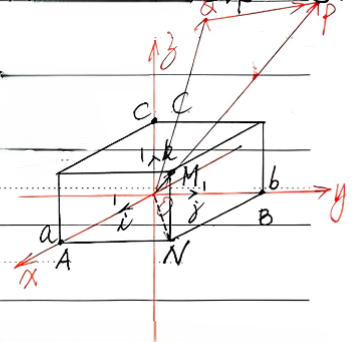
\includegraphics[width=0.5\textwidth]{figure/1-1空间直角坐标系.png}
    \caption{空间直角坐标系}
    \label{fig:fig1}
\end{figure}

\begin{definition}
    $\overrightarrow{OM}=(a,b,c)$,称$\sqrt{a^2+b^2+c^2}$为向量$\overrightarrow{OM}$的模,记为$\left|\overrightarrow{OM}\right|$.

    模长为$0$的向量为零向量$\0=(0,0,0)$,模长为$1$的向量称为单位向量.
\end{definition}
\begin{proposition}
    设向量$\balpha=(a,b,c)\neq \0$,则$\left|\balpha\right|\neq 0$.
    
    此时,$\balpha^0\triangleq\frac{\balpha}{\left|\balpha\right|}=\left(\frac{a}{\sqrt{a^2+b^2+c^2}},\frac{b}{\sqrt{a^2+b^2+c^2}},\frac{c}{\sqrt{a^2+b^2+c^2}}\right)$是单位向量.
\end{proposition}


\begin{remark}
\begin{enumerate}
    \item 这种定义方式较为依赖直观的几何性质,且可能存在一些循环定义的问题,当然针对这一阶段这样大概就足够了.
    \item 这种方式可以想见,是可以从三维向量(three-dimensional vector)推广至$n$维的,对应的向量就是$n$维向量(n-dimensional vector).
\end{enumerate}
\end{remark}
设$P=(x_1,y_1,z_1),Q=(x_1,y_1,z_1)$是空间的任意两点,$\overrightarrow{OP}=(x_1,y_1,z_1)$,$\overrightarrow{OQ}=(x_2,y_2,z_2)$.则$\overrightarrow{PQ}=(x_2,y_2,z_2)-(x_1,y_1,z_1)=(x\i+x_2\j+z_2\k)-(x_1\i+y_1\j+z_1\k)=(x_2-x_1)\i+(y_2-y_1)\j+(z_2-z_1)\k=(x_2-x_1,y_2-y_1,z_2-z_1)$.
即空间的任一个向量$\overrightarrow{PQ}=(x_2-x_1,y_2-y_1,z_2-z_1)$.

空间中的向量有无数个,但每一个都可用单位向量$\i,\j,\k$的线性组合来表示,称之前定义的$\i,\j,\k$为三维向量空间的标准正交基.

在任一个有限维的向量空间中,一旦选定了基向量,则"无限的问题便可有限化表示"了.

\begin{proposition}[三维数组向量的线性运算法则]
    设$\balpha=(a_1,b_1,c_1),\bbeta=(a_2,b_2,c_2),\lambda_1\in\R,\lambda_2\in\R$,则
    \begin{enumerate}
        \item 加、减法:$\balpha\pm\bbeta=(a_1\i+b_1\j+c_1\k)\pm(a_2\i+b_2\j+c_2\k)=(a_1\pm a_2)\i+(b_1\pm b_2)\j+(c_1\pm c_2)\k=(a_1\pm a_2,b_1\pm b_2,c_1\pm c_2)$.
        \item 数乘:$\lambda_1\balpha=\lambda_1(a_1\i+b_1\j+c_1\k)=(\lambda_1a_1)\i+(\lambda_1b_1)\j+(\lambda_1c_1)\k=(\lambda_1a_1,\lambda_1b_1,\lambda_1c_1)$.
    \end{enumerate}
    向量的加法、减法及数乘三种运算统称为向量的线性运算.统一为
    
    $\lambda_1\balpha+\lambda_2\bbeta=(\lambda_1a_1,\lambda_1b_1,\lambda_1c_1)+(\lambda_2a_2,\lambda_2b_2,\lambda_2c_2)=(\lambda_1a_1+\lambda_2a_2,\lambda_1b_1+\lambda_2b_2,\lambda_1c_1+\lambda_2c_2)$.
\end{proposition}

\section{向量的内积与外积}
\begin{definition}[内积与外积]
    设$\balpha=(a_1,b_1,c_1),\bbeta=(a_2,b_2,c_2)$.则
    \begin{enumerate}
        \item 内积: $\balpha\cdot\bbeta=\left|\balpha\right|\left|\bbeta\right|\cos(\widehat{\balpha,\bbeta})$
        \item 外积: $\balpha\times\bbeta$,满足$\begin{cases}
            \left|\balpha\times\bbeta\right|=\left|\balpha\right|\left|\bbeta\right|\sin(\widehat{\balpha,\bbeta})\\
            \balpha\times\bbeta\bot\balpha,\balpha\times\bbeta\bot\bbeta,\text{且}\balpha,\bbeta,\balpha\times\bbeta\text{构成右手系}.
        \end{cases}$
    \end{enumerate}
\end{definition}

\begin{figure}[h]
    \centering
    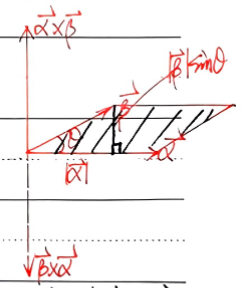
\includegraphics[width=0.5\textwidth]{figure/1-2外积的图示.png}
    \caption{外积的图示}
    \label{fig:fig2}
\end{figure}
\begin{remark}
    \begin{enumerate}
        \item $\balpha\cdot\bbeta$的规定来源于物理中里做功的运算,$\balpha\cdot\bbeta$是一个数,故称内积$\balpha\cdot\bbeta$为$\balpha$与$\bbeta$的数量积,或者称为点乘.
        \item $\balpha\times\bbeta$的规定来源于物理中的力矩的运算,$\balpha\times\bbeta$是一个向量,故称外积$\balpha\times\bbeta$为$\balpha$与$\bbeta$的向量积,或者称为叉乘.
    \end{enumerate}
\end{remark}

\begin{theorem}
    \begin{enumerate}
        \item $\balpha\bot\bbeta\Leftrightarrow\balpha\cdot\bbeta=0\Leftrightarrow a_1a_2+b_1b_2+c_1c_2=0$.
        \item $\balpha\parallel\bbeta\Leftrightarrow\balpha\times\bbeta=\0\Leftrightarrow\frac{a_1}{a_2}=\frac{b_1}{b_2}=\frac{c_1}{c_2}\Leftrightarrow \balpha=\lambda\bbeta$
    \end{enumerate}
\end{theorem}
\begin{proof}
    \begin{enumerate}
        \item 
        \begin{enumerate}[1)]
            \item 若$\balpha\bot\bbeta$,则$\cos(\widehat{\balpha,\bbeta})=0\Rightarrow\balpha\cdot\bbeta=\left|\balpha\right|\left|\bbeta\right|\cos(\widehat{\balpha,\bbeta})=0$.            
            \item 反之,若$\balpha\cdot\bbeta=0$,则$\left|\balpha\right|\left|\bbeta\right|\cos(\widehat{\balpha,\bbeta})=0$,若$\left|\balpha\right|\left|\bbeta\right|\neq 0$,则$\cos(\widehat{\balpha,\bbeta})=0$,从而$\balpha\bot\bbeta$.若$\left|\balpha\right|\left|\bbeta\right|=0$,则$\balpha=\0$或$\bbeta=\0$,由于零向量$\0$垂直于任意向量,故$\balpha\bot\bbeta$.
            \item $\balpha\cdot\bbeta=(a_1\i+b_1\j+c_1\k)\cdot(a_2\i+b_2\j+c_2\k)=a_1a_2\i\cdot\i+a_1b_2\i\cdot\j+a_1c_2\i\cdot\k+b_1a_2\j\cdot\i+b_1b_2\j\cdot\j+b_1c_2\j\cdot\k+c_1a_2\k\cdot\i+c_1b_2\k\cdot\j+c_1c_2\k\cdot\k.\text{而}\i\cdot\i=\left|\i\right|\left|\i\right|\cos(\widehat{\i,\i})=1\times1\times\cos0=1=\j\cdot\j=\k\cdot\k,\text{且由于}\i\bot\j,\i\bot\k,\j\bot\k,\text{故}\i\cdot\j=\i\cdot\k=\j\cdot\k=0,\text{故}\balpha\cdot\bbeta=a_1a_2+b_1b_2+c_1c_2$.
        \end{enumerate}
        \item
        \begin{enumerate}[1)]
            \item 若$\balpha\parallel\bbeta$,则$\sin(\widehat{\balpha,\bbeta})=0\Rightarrow\left|\balpha\times\bbeta\right|=\left|\balpha\right|\left|\bbeta\right|\sin(\widehat{\balpha,\bbeta})=0\Rightarrow\balpha\times\bbeta=\0$.
            \item 反之,若$\balpha\times\bbeta=\0$,则$\left|\balpha\times\bbeta\right|=\left|\0\right|=0=\left|\balpha\right|\left|\bbeta\right|\sin(\widehat{\balpha,\bbeta})$,若$\left|\balpha\right|\left|\bbeta\right|\neq 0$,则$\sin(\widehat{\balpha,\bbeta})=0$,从而$\balpha\parallel\bbeta$.若$\left|\balpha\right|\left|\bbeta\right|=0$,则$\balpha=\0$或$\bbeta=\0$,由于零向量$\0$平行于任意向量,故$\balpha\parallel\bbeta$.
            \item $
            \begin{cases}
                \i\times\i=\0,\j\times\j=\0,\k\times\k=\0\\
                \i\times\j=\k,\j\times\i=-\k,\j\times\k=\i\\
                \k\times\j=-\i,\k\times\i=\j,\i\times\k=-\j
            \end{cases}$
            $\Rightarrow \balpha\times\bbeta=(a_1\i+b_1\j+c_1\k)\times(a_2\i+b_2\j+c_2\k)=a_1a_2\i\times\i+a_1b_2\i\times\j+a_1c_2\i\times\k+b_1a_2\j\times\i+b_1b_2\j\times\j+b_1c_2\j\times\k+c_1a_2\k\times\i+c_1b_2\k\times\j+c_1c_2\k\times\k=a_1b_2\k-a_1c_2\j-b_1a_2\k+b_1c_2\i+c_1a_2\j-c_1b_2\i=(b_1c_2-c_1b_2)\i-(a_1c_2-c_1a_2)\j+(a_1b_2-b_1a_2)\k=\begin{matrix}
                \begin{vmatrix}
                    \i&\j&\k\\
                    a_1&b_1&c_1\\
                    a_2&b_2&c_2
                \end{vmatrix}
            \end{matrix}$.
            由$bf{\alpha}\parallel\bbeta\Leftrightarrow\balpha\times\bbeta=\0=(0,0,0)\Leftrightarrow\begin{cases}
                b_1c_2-c_1b_2=0\\
                c_1a_2-a_1c_2=0\\
                a_1b_2-b_1a_2=0
            \end{cases}
            \Leftrightarrow \frac{a_1}{a_2}=\frac{b_1}{b_2}=\frac{c_1}{c_2}\triangleq\lambda$.
            因此可得$\balpha=\lambda\bbeta$.
        \end{enumerate}
    \end{enumerate}
\end{proof}
\begin{remark}
    \begin{enumerate}
        \item 在上述证明中,不加证明地使用了点乘与叉乘的分配率等性质.
        \item 与证明中提到的类似,点乘有坐标表达$\balpha\cdot\bbeta=a_1a_2+b_1b_2+c_1c_2$,叉乘有坐标表达$\balpha\times\bbeta=\begin{matrix}
            \begin{vmatrix}
                \i&\j&\k\\
                a_1&b_1&c_1\\
                a_2&b_2&c_2
            \end{vmatrix}\end{matrix}$,     
        这也是最常用的计算公式.
    \end{enumerate}
\end{remark}

\section{例题}
    设$\balpha=(a_1,b_1,c_1),\bbeta=(a_2,b_2,c_2),\bgamma=(a_3,b_3,c_3)$.
\begin{example}
    证明:柯西不等式$\left|a_1a_2+b_1b_2+c_1c_2\right|\les\sqrt{a_1^2+b_1^2+c_1^2}\sqrt{a_2^2+b_2^2+c_2^2}$.
\end{example}

\begin{proof}
    $\left|a_1a_2+b_1b_2+c_1c_2\right|=\left|\balpha\cdot\bbeta\right|=\left|\balpha\right|\left|\bbeta\right|\cos(\widehat{\balpha,\bbeta})\les\left|\balpha\right|\left|\bbeta\right|=\sqrt{a_1^2+b_1^2+c_1^2}\sqrt{a_2^2+b_2^2+c_2^2}$.
\end{proof}

\begin{remark}
    在$n$维向量空间中,设$\balpha=(a_1,a_2,\cdots,a_n),\bbeta=(b_1,b_2,\cdots,b_n)$,则$\left|\balpha\cdot\bbeta\right|=\left|\balpha\right|\left|\bbeta\right|\cos(\widehat{\balpha,\bbeta})\les\left|\balpha\right|\left|\bbeta\right|$,即$\left|a_1b_1+a_2b_2+\cdots+a_nb_n\right|\les\sqrt{a_1^2+a_2^2+\cdots+a_n^2}\sqrt{b_1^2+b_2^2+\cdots+b_n^2}$.
\end{remark}

\begin{example}
    证明:$\left|\balpha\times\bbeta\right|^2=\left|\balpha\right|^2\left|\bbeta\right|^2-\left|\balpha\cdot\bbeta\right|^2$.
\end{example}
\begin{proof}
    $\left|\balpha\times\bbeta\right|^2=\left|\balpha\right|^2\left|\bbeta\right|^2\sin^2(\widehat{\balpha,\bbeta})=\left|\balpha\right|^2\left|\bbeta\right|^2(1-\cos^2(\widehat{\balpha,\bbeta}))=\left|\balpha\right|^2\left|\bbeta\right|^2-\left|\balpha\right|^2\left|\bbeta\right|^2\cos^2(\widehat{\balpha,\bbeta})=\left|\balpha\right|^2\left|\bbeta\right|^2-\left|\balpha\cdot\bbeta\right|^2$.
\end{proof}

\begin{example}
    证明:$(\balpha\times\bbeta)\cdot\bgamma=(\bbeta\times\bgamma)\cdot\balpha=(\bgamma\times\balpha)\cdot\bbeta$.
\end{example}
\begin{proof}
    $(\balpha\times\bbeta)\cdot\bgamma=\begin{matrix}
        \begin{vmatrix}
            \i&\j&\k\\
            a_1&b_1&c_1\\
            a_2&b_2&c_2
        \end{vmatrix}
    \end{matrix}\cdot(a_3\i+b_3\j+c_3\k)=((b_1c_2-c_1b_2)\i+(c_1a_2-a_1c_2)\j+(a_1b_2-a_2b_1)\k)\cdot(a_3\i+b_3\j+c_3\k)=(b_1c_2-c_1b_2)a_3+(c_1a_2-a_1c_2)b_3+(a_1b_2-a_2b_1)c_3=\begin{matrix}
        \begin{vmatrix}
            a_1&b_1&c_1\\
            a_2&b_2&c_2\\
            a_3&b_3&c_3
        \end{vmatrix}
    \end{matrix}=(\bbeta\times\bgamma)\cdot\balpha=(\bgamma\times\balpha)\cdot\bbeta$.
\end{proof}

\begin{example}
    证明:三个向量$\balpha,\bbeta,\bgamma$共面的充要条件是$(\balpha\times\bbeta)\cdot\bgamma=0$.
\end{example}
\begin{proof}
    是如下结论的结果:如图所示,根据计算公式,$\left|\balpha\times\bbeta\right|$是以$\balpha$和$\bbeta$为两边的平行四边形的面积,而$\bgamma\left|\cos(\widehat{\balpha\times\bbeta,\bgamma})\right|$是$\bgamma$在垂直于平行四边形方向上的投影,即$h=\left|\bgamma\right|\left|\cos(\widehat{\balpha\times\bbeta,\bgamma})\right|$,因此$(\balpha\times\bbeta)\cdot\bgamma$是以$\balpha$, $\bbeta$和$\bgamma$为三边的平行六面体的体积,于是$\balpha,\bbeta,\bgamma$共面$\Leftrightarrow$平行六面体的体积为$0$ $\Leftrightarrow(\balpha\times\bbeta)\cdot\bgamma=\begin{matrix}
        \begin{vmatrix}
            a_1&b_1&c_1\\
            a_2&b_2&c_2\\
            a_3&b_3&c_3
        \end{vmatrix}
    \end{matrix}=0$.
\end{proof}

\begin{figure}[h]
    \centering
    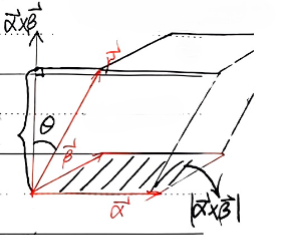
\includegraphics[width=0.5\textwidth]{figure/1-3混合积与平行六面体.png}
    \caption{混合积与平行六面体}
    \label{fig:fig3}
\end{figure}
\begin{example}
    $\forall \lambda_1,\lambda_2\in\R$总有$\balpha,\bbeta,\lambda_1\balpha+\lambda_2\bbeta$共面.
\end{example}
\begin{proof}
    利用$\balpha\bot\balpha\times\bbeta,\bbeta\bot\balpha\times\bbeta$,则$(\balpha\times\bbeta)\cdot\balpha=0,(\balpha\times\bbeta)\cdot\bbeta=0$,从而$(\balpha\times\bbeta)\cdot(\lambda_1\balpha+\lambda_2\bbeta)=0$,因此可得$\balpha,\bbeta,\lambda_1\balpha+\lambda_2\bbeta$共面.
\end{proof}

\begin{homework} 
    ex8.1:6,9,10,12,14,17,23,26.
\end{homework}